\documentclass[a4paper, 12pt, titlepage]{article}
\usepackage{graphicx}
\usepackage{titlesec}
\usepackage{hyperref}
\usepackage{float}
\usepackage{chngcntr}
\counterwithin{table}{section}
\usepackage{amsmath}
\numberwithin{figure}{section}
\graphicspath{{Images/}}
\usepackage{listings}
\usepackage{hhline}
\usepackage{longtable}

%cost driver
\newenvironment{costdriverstable}[1]{
	\setlength{\LTleft}{-40pt}
	\begin{longtable}{|p{\dimexpr.16\textwidth}|p{\dimexpr.14\textwidth}|p{\dimexpr.14\textwidth}|p{\dimexpr.14\textwidth}|p{\dimexpr.14\textwidth}|p{\dimexpr.14\textwidth}|p{\dimexpr.14\textwidth}|}
	\hline
	\multicolumn{7}{|c|}{{#1}}\\\hhline{|=======|}
}{
	\hline\end{longtable}
}

\newcommand{\costdescriptors}[7]{
	#1 & #2 & #3 & #4 & #5 & #6 & #7\\
}

\newcommand{\ratinglevel}[6]{
	Rating level & #1 & #2 & #3 & #4 & #5 & #6 \\\hline
}

\newcommand{\effortmultipliers}[6]{
	Effort multipliers & #1 & #2 & #3 & #4 & #5 & #6 \\\hline
}

%scale driver
%  table
\newenvironment{scaledriverstable}[1]{
	\setlength{\LTleft}{-40pt}
	\begin{center}
	#1 
	\begin{longtable}{|p{\dimexpr.16\textwidth}|p{\dimexpr.14\textwidth}|p{\dimexpr.14\textwidth}|p{\dimexpr.14\textwidth}|p{\dimexpr.14\textwidth}|p{\dimexpr.14\textwidth}|p{\dimexpr.14\textwidth}|}
	\hline
}{
	\hline\end{longtable}\end{center}
}


%scale driver command
\newcommand{\addfactor}[7]{
	#1 & #2 & #3 & #4 & #5 & #6 & #7 \\
}
\newcommand{\addfactorvalues}[6]{
SF$_j$ & #1 & #2 & #3 & #4 & #5 & #6 \\\hline
}

% Table cells spanning multiple rows
\usepackage{multirow}

% Subfigures and subtables
\usepackage{subcaption}

%subsubsubsection
\titleclass{\subsubsubsection}{straight}[\subsection]

\newcounter{subsubsubsection}[subsubsection]
\renewcommand\thesubsubsubsection{\thesubsubsection.\arabic{subsubsubsection}}
\renewcommand\theparagraph{\thesubsubsubsection.\arabic{paragraph}} % optional; useful if paragraphs are to be numbered

\titleformat{\subsubsubsection}
{\normalfont\normalsize\bfseries}{\thesubsubsubsection}{1em}{}
\titlespacing*{\subsubsubsection}
{0pt}{3.25ex plus 1ex minus .2ex}{1.5ex plus .2ex}

\makeatletter
\renewcommand\paragraph{\@startsection{paragraph}{5}{\z@}%
	{3.25ex \@plus1ex \@minus.2ex}%
	{-1em}%
	{\normalfont\normalsize\bfseries}}
\renewcommand\subparagraph{\@startsection{subparagraph}{6}{\parindent}%
	{3.25ex \@plus1ex \@minus .2ex}%
	{-1em}%
	{\normalfont\normalsize\bfseries}}
\def\toclevel@subsubsubsection{4}
\def\toclevel@paragraph{5}
\def\toclevel@paragraph{6}
\@addtoreset{subsubsubsection}{section}
\@addtoreset{subsubsubsection}{subsection}
\def\l@subsubsubsection{\@dottedtocline{4}{7em}{4em}}
\def\l@paragraph{\@dottedtocline{5}{10em}{5em}}
\def\l@subparagraph{\@dottedtocline{6}{14em}{6em}}
\makeatother
%end
\setcounter{secnumdepth}{4}
\setcounter{tocdepth}{4}
\hypersetup{
	colorlinks=true,
	linkcolor=black,
	filecolor=magenta,      
	urlcolor=cyan,
}
%opening
\title{
	\begin{figure}[h]
		\centering
		
\includegraphics{images/polimi_logo.jpg}
	\end{figure}
	Politecnico di Milano, A.A. 2016/2017 
	\newline\newline 
	Software Engineering 2: PowerEnJoy \\
	Project Plan}
\author{Binosi Lorenzo 876022}
	
	
\begin{document}
	
	\maketitle
	\tableofcontents
	\newpage
	
	\section{Introduction} \label{sec introduction}


\subsection{Purpose}

The Design Document has the purpose to provide a functional description of the system. It defines the design of the software architecture, its components and their interactions, provided with the used algorithms and the user interfaces design. 

The document is written for project managers, developers, testers and quality assurance. It can be used for a structural overview to help maintenance and further development.


\subsection{Scope}

PowerEnJoy is a large-scale car-sharing service. It requires to perform excellently, to be secure, easily modifiable and as available as possible. Minding these necessities, in the following chapters will be shown how the system is structured and and which were the reasons that led to such decisions.
  
\subsection{Definitions, Acronyms, Abbreviations}

\begin{description}
	\item[DD:] Design Document.
	\item[RASD:] Requirements Analysis and Specification Document.
	\item[System:] the whole software system to be developed, comprehensive of all its parts.
	\item[REST:] REpresentational State Transfer. It's an architectural style and an approach to stateless communications, used in the development of client-server systems.
	\item[GUI:] Graphical User Interface.
	\item[ACID:] Atomicity, Consistency, Isolation, Durability. A set of properties of database transactions.
	\item[API:] Application Programming Interface.
	\item[EJB:] Enterprise Java Bean.
	\item[JPA:] Java Persistence API.
	\item[JSP:] JavaServer Pages.
	\item[HTTP:] HyperText Transfer Protocol.
	\item[HTTPS:] HyperText Transfer Protocol Secure.
\end{description}

\subsection{Reference Documents}

This document refers to the project rules of the Software Engineering 2 project~\cite{se-project-rules} and to the DD assignment~\cite{se-assignment}.

\subsection{Document Structure}

This document is structured in five parts:
\begin{description}
	\item[\autoref{sec introduction}: Introduction.] This section provides general information about the DD document and the used terms.
	\item[\autoref{sec architectural design}: Architectural Design.] This section shows the software architecture of the system, with its components and their interactions.
	\item[\autoref{sec algorithm design}: Algorithm Design.] This section will present and discuss in detail the algorithms designed for the system functionalities, independently from their concrete implementation.
	\item[\autoref{sec user interface design}: User Interface Design.] This section shows how the user interface will look like and behave, by means of concept graphics and UX modeling.
	\item[\autoref{sec requirements traceability}: Requirements Traceability.] shows how the requirements in the RASD~\cite{rasd} are satisfied by the design choices of the DD.
\end{description}
	
	\section{Project size, cost and effort estimation}

This section describes which are the main functionalities of PowerEnJoy that allowed us to estimate the expected size, the cost and the required effort of the project. 

For the size estimation we will use the \textbf{Function Points} approach. It allows to estimate the correspondent amount of lines of code to be written in Java, according to the main functionalities of PowerEnJoy. We won't consider the functionalies of the user interface in order to have a more meaningful and reliable estimation.

For the cost and effort estimation we will use the \textbf{COCOMO II} model, relying on the amount of lines of code estimated previously.

\subsection{Size estimation}

For the size estimation we will refer to the IFPUG 1994 standard~\cite{ifpug} which specifies the definitions, rules and steps for applying the IFPUG's functional size measurement (FSM) method.

In order to determine the complexity level, the IFPUG standard classifies each function count into Low, Average and High complexity levels depending on the number of data element types contained and the number of file types referenced. Tables \ref{tab:complexity-estimation1},  \ref{tab:complexity-estimation2} and \ref{tab:complexity-estimation3} reassume the complexity levels for each type of file. 

Once determined the complexity of each function, it's possible to define its weight, i.e., the relative effort required to implement it. Table \ref{tab:complexity-weights} reassume the Unadjusted Function Points (UFP) for each complexity level.

\begin{table}[H]
\centering
\begin{subtable}{\textwidth}
    \centering
    \begin{tabular}{| c | l | l | l |}
        \hline
         & \multicolumn{3}{c|}{\textbf{Data Elements}} \\
        \hline
        \textbf{Record Elements} & 1-19 & 20-50 & 51+ \\
        \hline
        1       & Low     & Low     & Avg.     \\
        2-5    & Low     & Avg.    & High     \\
        6+     & Avg.    & High    & High     \\
        \hline
    \end{tabular}
    \caption{Complexity estimation for ILFs and EIFs.}
    \label{tab:complexity-estimation1}
\end{subtable}

\vspace{2em}

\begin{subtable}{\textwidth}
    \centering
    \begin{tabular}{| c | l | l | l |}
        \hline
         & \multicolumn{3}{c|}{\textbf{Data Elements}} \\
        \hline
        \textbf{Record Elements} & 1-5 & 6-19 & 20+ \\
        \hline
        0-1     & Low     & Low     & Avg.     \\
        2-3     & Low     & Avg.    & High     \\
        4+      & Avg.    & High    & High     \\
        \hline
    \end{tabular}
    \caption{Complexity estimation for EOs and EQs.}
    \label{tab:complexity-estimation2}
\end{subtable}

\vspace{2em}

\begin{subtable}{\textwidth}
    \centering
    \begin{tabular}{| c | l | l | l |}
        \hline
         & \multicolumn{3}{c|}{\textbf{Data Elements}} \\
        \hline
        \textbf{Record Elements} & 1-4 & 5-15 & 16+ \\
        \hline
        1       & Low     & Low     & Avg.     \\
        2-3     & Low     & Avg.    & High     \\
        3+      & Avg.    & High    & High     \\
        \hline
    \end{tabular}
    \caption{Complexity estimation for EIs.}
    \label{tab:complexity-estimation3}
\end{subtable}
\caption{Estimation of complexities for different types of Function Points.}
\label{tab:complexity-estimation}
\end{table}

\begin{table}[H]
    \centering
    \begin{tabular}{| l | l | l | l |}
        \hline
        \multirow{2}{*}{\textbf{Function Type}} & \multicolumn{3}{c|}{\textbf{Complexity-Weight}} \\
        \cline{2-4}
        & Low & Average & High \\
        \hline
        Internal Logic Files    & 7     & 10    & 15    \\
        External Interface Files & 5     & 7     & 10    \\
        External Inputs          & 3     & 4     & 6     \\
        External Outputs       & 4     & 5     & 7     \\
        External Inquiries        & 3     & 4     & 6     \\
        \hline
    \end{tabular}
    \caption{UFP complexity weights.}
    \label{tab:complexity-weights}
\end{table}

\newpage 

\subsubsection{Internal Logic Files (ILFs)}

The ILFs are those logical files generated, used or mantained by the software system. In our case they include all the information that the system has to store:
\begin{itemize}
	\item Driver:
	\begin{itemize}
		\item Driver information
		\item CreditCard
	\end{itemize}
	\item Rent:
	\begin{itemize}
		\item Rental information
		\item RentalEvents
	\end{itemize}
	\item Car
	\item SafeArea
	\item CarAssistance
\end{itemize}
The Driver Record Element (RET) contains 15 Data Elements (DET's) and the CreditCard RET, which contains 2 DET's. Hence, according to the Table \ref{tab:complexity-estimation}, the Driver ILF has a low complexity with an amount of 2 RET's and 17 DET's.

The Rent RET contains 6 DET's  and the RentalEvent RET, which contains 2 DET's. Hence, the Rent ILF has a low complexity with an amount of 2 RET's and 8 DET's.

The Car, SafeArea and CarAssistance RET's contain respectively 11, 4 and 4 DET's, and their ILFs have a low complexity.

\vspace{2em}

\begin{table}[H]
    \centering
    \begin{tabular}{| l | l | l |}
        \hline
        \textbf{ILF} & \textbf{Complexity} & \textbf{FPs} \\
        \hline
        Driver           & Low     & 7     \\
        Rent           & Low     & 7     \\
        Car           & Low     & 7     \\
        SafeArea           & Low     & 7     \\
        CarAssistance           & Low     & 7     \\
        \hline
        \multicolumn{2}{| l |}{\textbf{Total}}  & \textbf{35} \\
        \hline
    \end{tabular}
    \caption{The ILFs complexity and the total Function Points.}
    \label{tab:computed-num-weights}
\end{table}

\subsubsection{External Interface Files (EIFs)}

PowerEnJoy needs to interface with 3 services, described in the DD, in order to perform some operations. They are:
\begin{description}
	\item[SMSGateway]: for the SMS dispatching.
	\item[EmailSender]: for the email dispatching.
	\item[PaymentGateway]: for the payment execution.	
\end{description}
Obviously, each of these services doesn't require too much data, so we can consider their complexity as low.

\vspace{2em}

\begin{table}[H]
    \centering
    \begin{tabular}{| l | l | l |}
        \hline
        \textbf{ELF} & \textbf{Complexity} & \textbf{FPs} \\
        \hline
        SMSGateway           & Low     & 5     \\
        EmailSender           & Low     & 5     \\
        PaymentGateway           & Low     & 5     \\
        \hline
        \multicolumn{2}{| l |}{\textbf{Total}}  & \textbf{15} \\
        \hline
    \end{tabular}
    \caption{The ELFs complexity and the total Function Points.}
    \label{tab:computed-num-weights}
\end{table}

\subsubsection{External Inputs (EIs) and External Inquiries (EQs)}

The PowerEnJoy business logic provides a RESTful API for all the core functionalities of the system. All the API requests are completely described in the DD [2.5.3, p. 14] and summarized below. Thanks to this detailed description, the complexity estimation of the EIs and the EQs will be performed accurately.

\begin{itemize}
	\item User creation: this request allows the creation of a new user. It requires all the user information as input and doesn't provide any output data. According to Table \ref{tab:complexity-estimation3}, the EI of the request has an high complexity with an amount of 3 RET's and 12 DET's.
	\item User's salt bytes retrieval: this request allows to retrieve the user's salt bytes in order to use them for the password hashing. It requires only the username of the user as input and provides the user's salt bytes as output. The EI and the EQ of the request have both a low complexity.
	\item User deletion: this request allows to delete the user that performs the request. It requires only the credentials of the user (username and hashed password) as input and doesn't provide any output data. The EI of the request has a low complexity.
	\item User's rental logbook retrieval: this request allows a user to retrieve his/her rental logbook. It requires only the credentials of the user as input and provides the logbook information as output. The EI and the EQ of the request have respectively a low and a medium complexity. In particular we can observe that the EQ contains an amount of 2 RET's and 6 DET's which give the medium complexity, according to Table \ref{tab:complexity-estimation2}.
	\item Available cars' retrieval: this request allows a user to retrieve all the available cars in the nearby area. It requires the credentials of the user and his/her geographical position as input, and provides the data about the available cars as output. The EI and the EQ of the request have respectively a low and a medium complexity. In particular we can observe thath the EQ cointains an amount of 3 RET's and 6 DET's which give the medium complexity
	\item Car reservation: this request allows a user to reserve a choosen car. It requires the credentials of the user and the license plate of the car as input, and doesn't provide any output data. The EI of the request has a low complexity.
	\item Current reservation retrieval:
\end{itemize}


	
	\section{Tasks and schedule}

In this section we are going to provide which are the tasks and the subtasks required by the project to be completed. For the documentation, which includes RASD, DD, ITPD and PP, we will consider the deadlines given by the Software Engneering 2 course and, for all that concern the development and the post-development, we will consider the immediately following period.

The final schedule is now summarized and completely described in the following figures.

\begin{itemize}
	\item RASD [04/10/2016 - 13/11/2016]
	\item DD [14/11/2016 - 11/12/2016]
	\item ITPD [12/12/2016 - 15/01/2017]
	\item PP [16/01/2017 - 22/01/2017]
	\item Documents review [23/01/2017 - 21/02/2017]
	\item Presentation [22/01/2017]
	\item Development [23/01/2017 - 25/08/2017]
	\item Deployment [26/08/2017 - 10/10/2017]
	\item Maintenance [11/10/2017 - undetermined]
\end{itemize}

\begin{figure}[H]
	\centering
	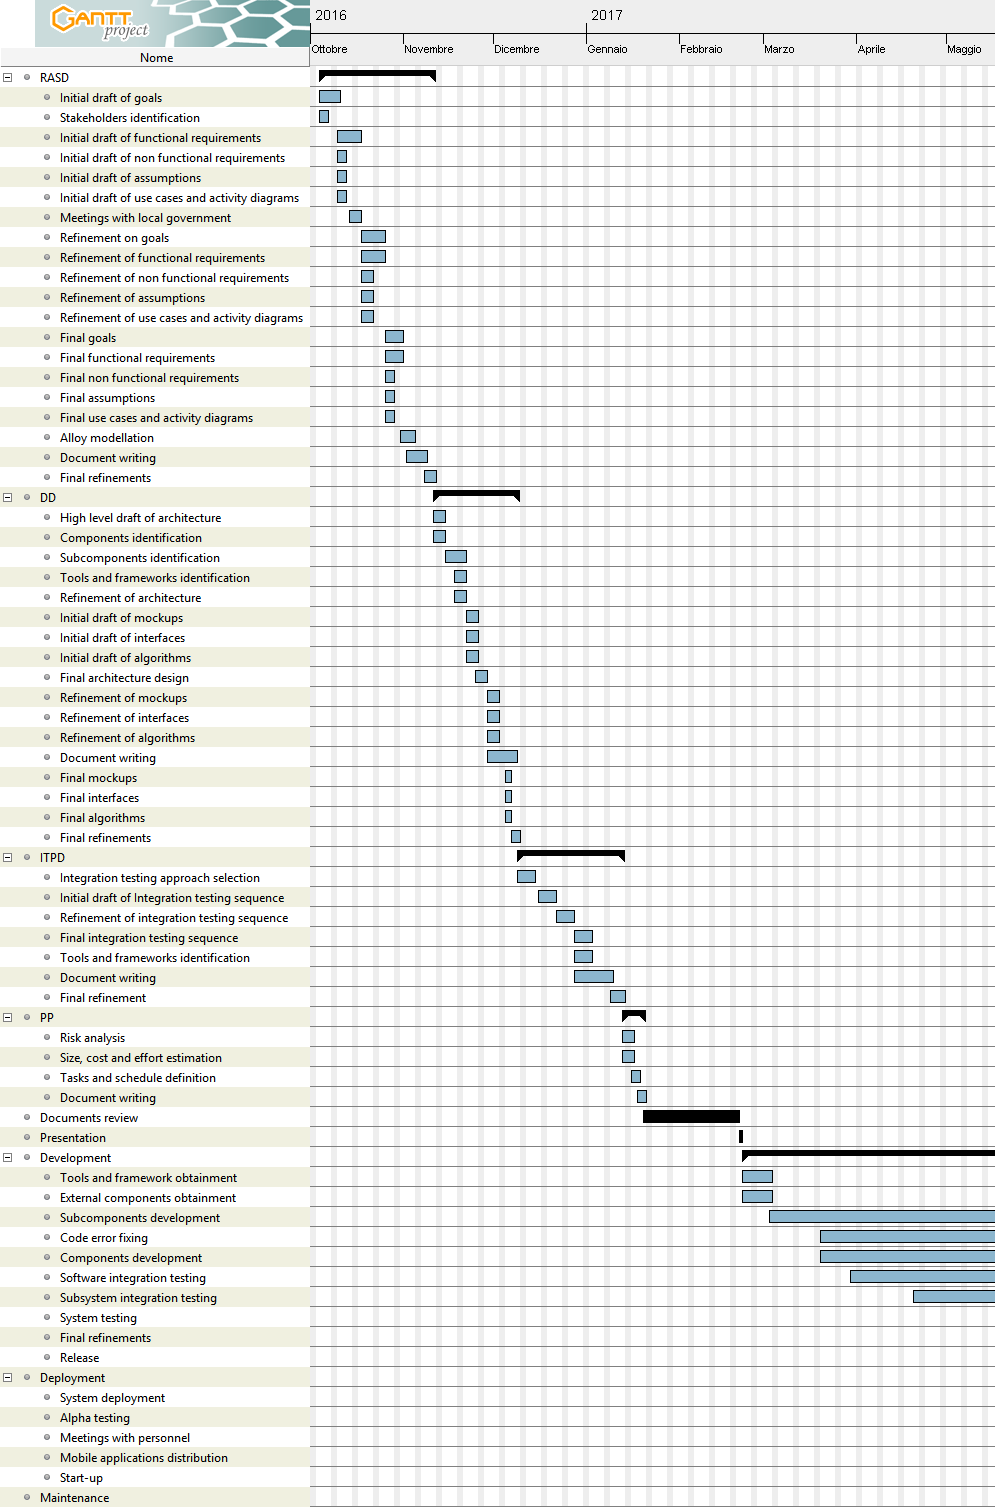
\includegraphics[width=\textwidth, keepaspectratio]{task_and_schedule/diagrams/Tasks1.png}
\end{figure}

\begin{figure}[H]
	\centering
	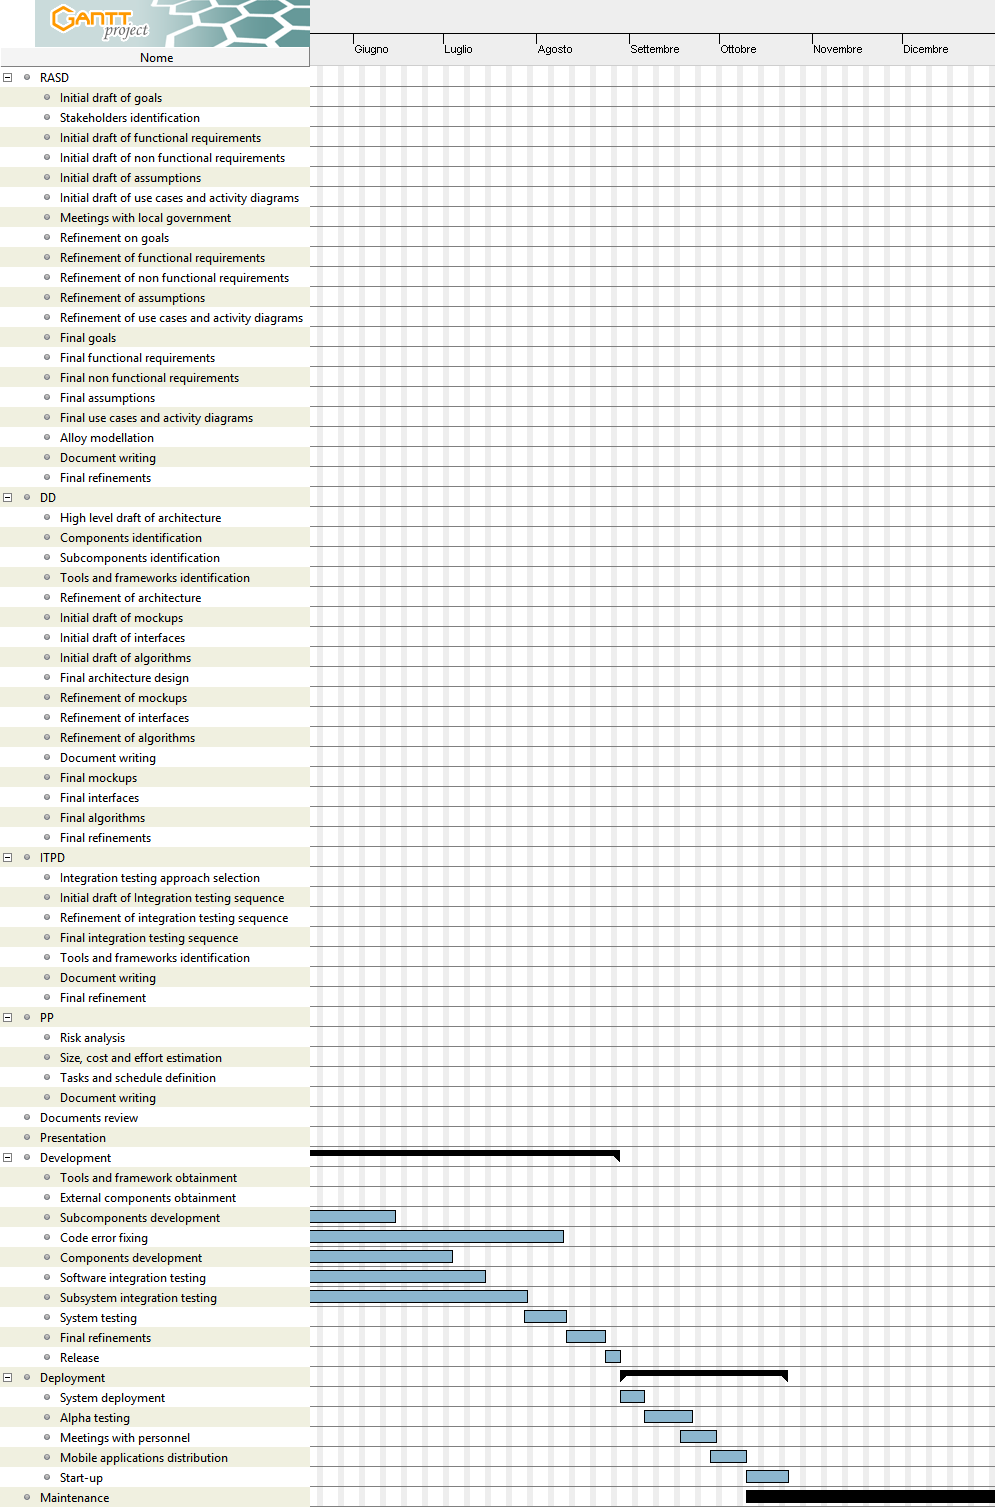
\includegraphics[width=\textwidth, keepaspectratio]{task_and_schedule/diagrams/Tasks2.png}
\end{figure}

	\section{Resource allocation}

In this section we are going to provide a possible resources allocation for the schedule defined in the previous section. Tasks and subtasks will be divided between the three member of our team, i.e., our resources, which have been introduced in Section \ref{cost-effort-est}.

It's important to note that a subtask could be performed by all the members of the team because, the decisions made and the knowledge obtained at the completion of the subtask, could be essential in order to perform other subtasks.

\begin{figure}[H]
	\centering
	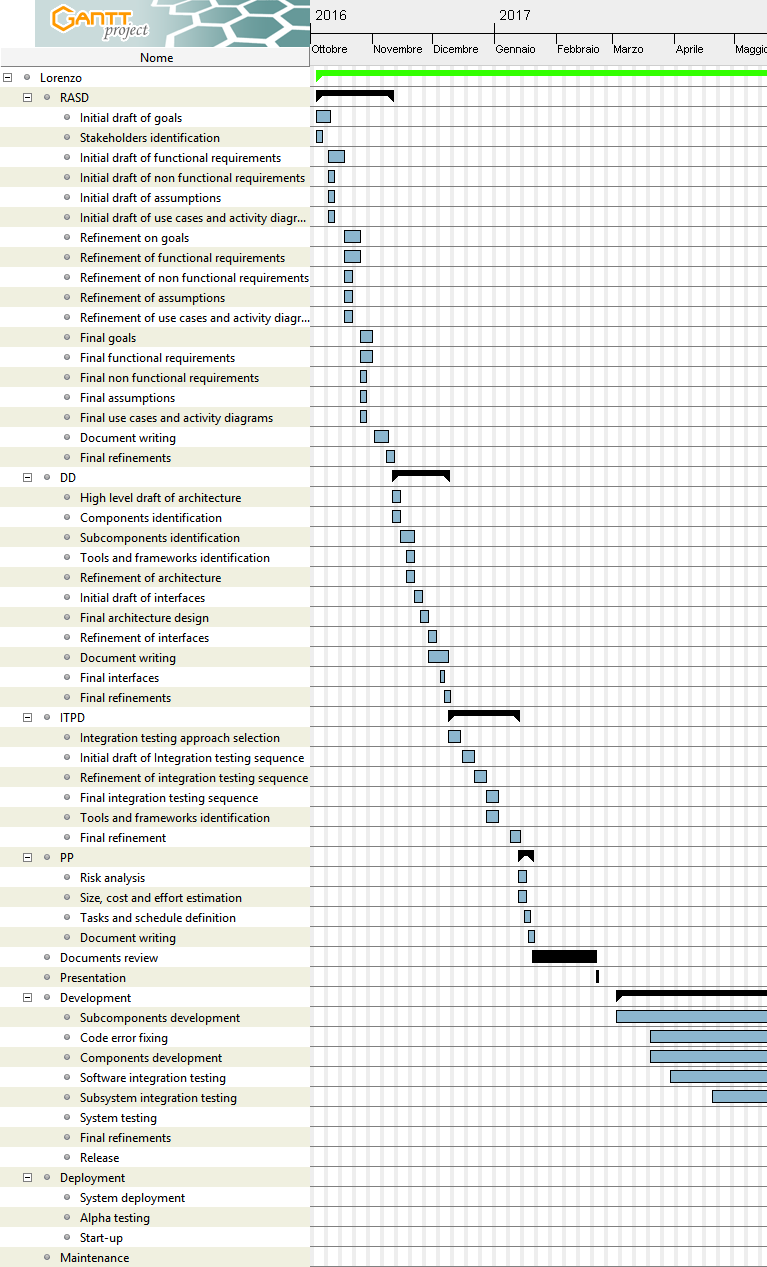
\includegraphics[height=\textheight, keepaspectratio]{resource_allocation/diagrams/ScheduleLorenzo1.png}
\end{figure}

\begin{figure}[H]
	\centering
	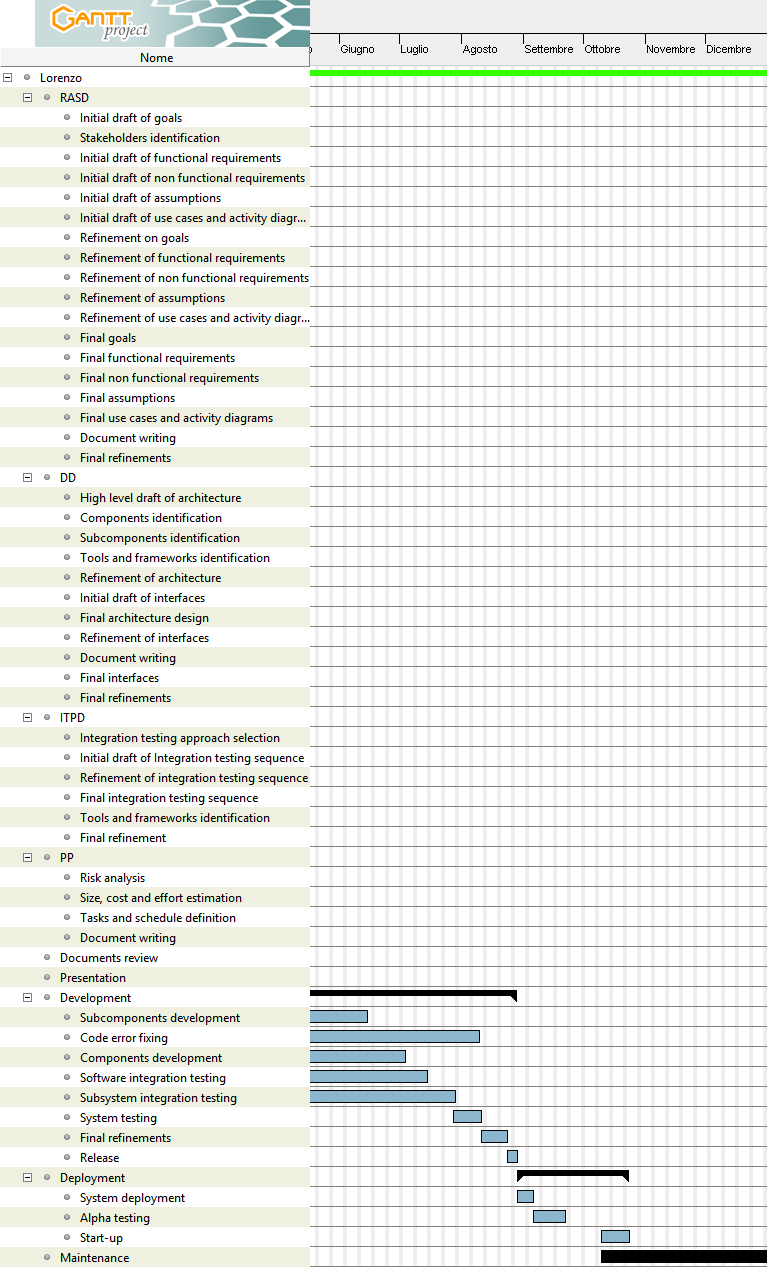
\includegraphics[height=\textheight, keepaspectratio]{resource_allocation/diagrams/ScheduleLorenzo2.png}
\end{figure}

\begin{figure}[H]
	\centering
	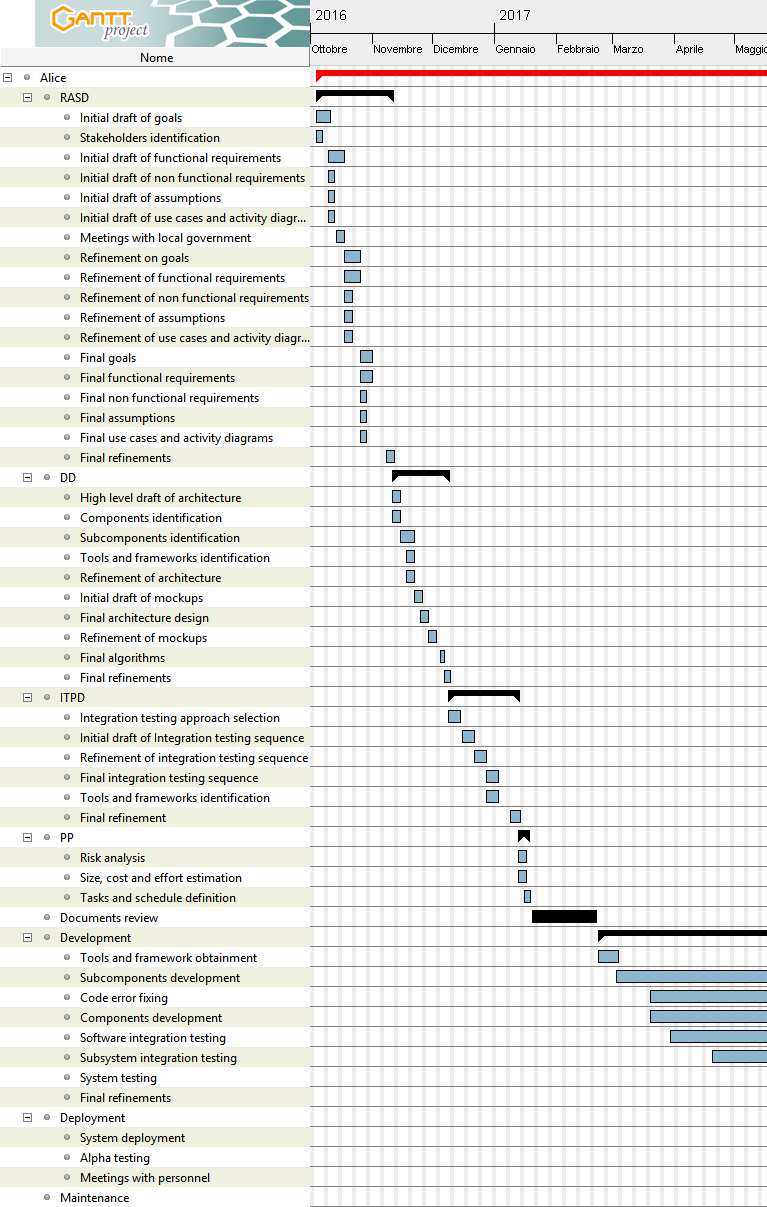
\includegraphics[height=\textheight, keepaspectratio]{resource_allocation/diagrams/ScheduleAlice1.png}
\end{figure}

\begin{figure}[H]
	\centering
	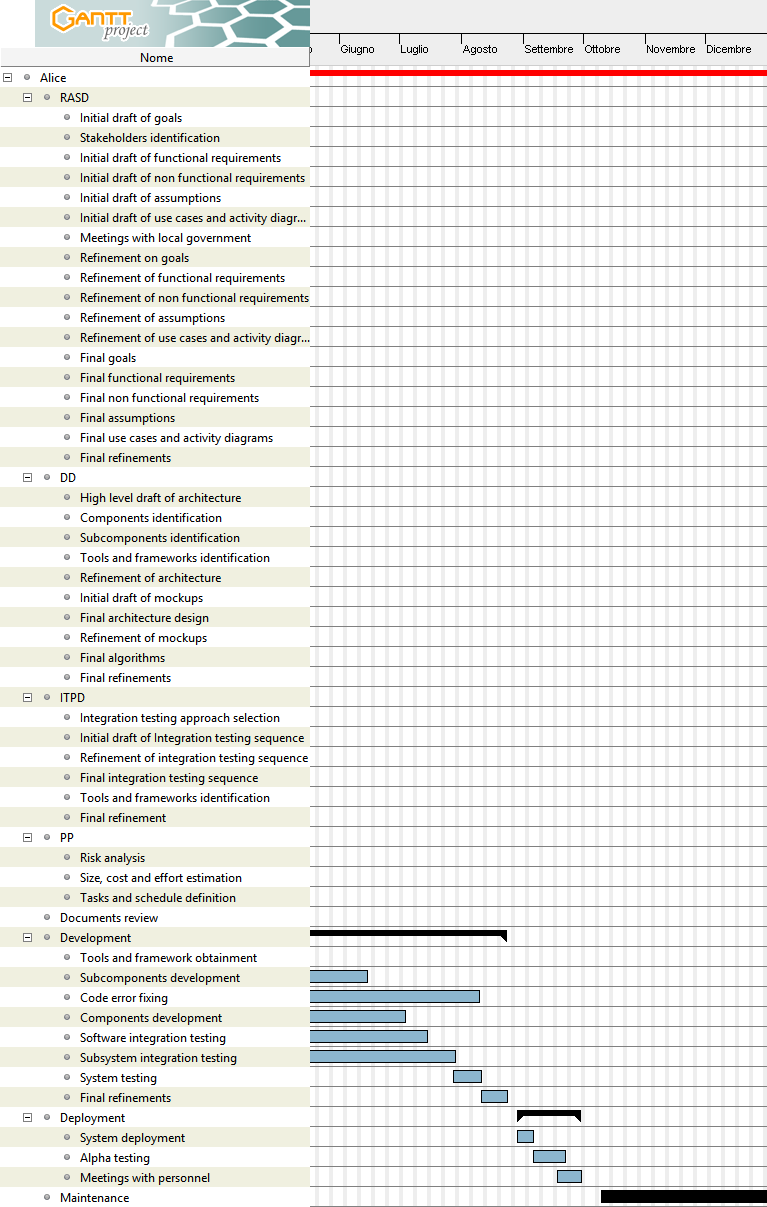
\includegraphics[height=\textheight, keepaspectratio]{resource_allocation/diagrams/ScheduleAlice2.png}
\end{figure}

\begin{figure}[H]
	\centering
	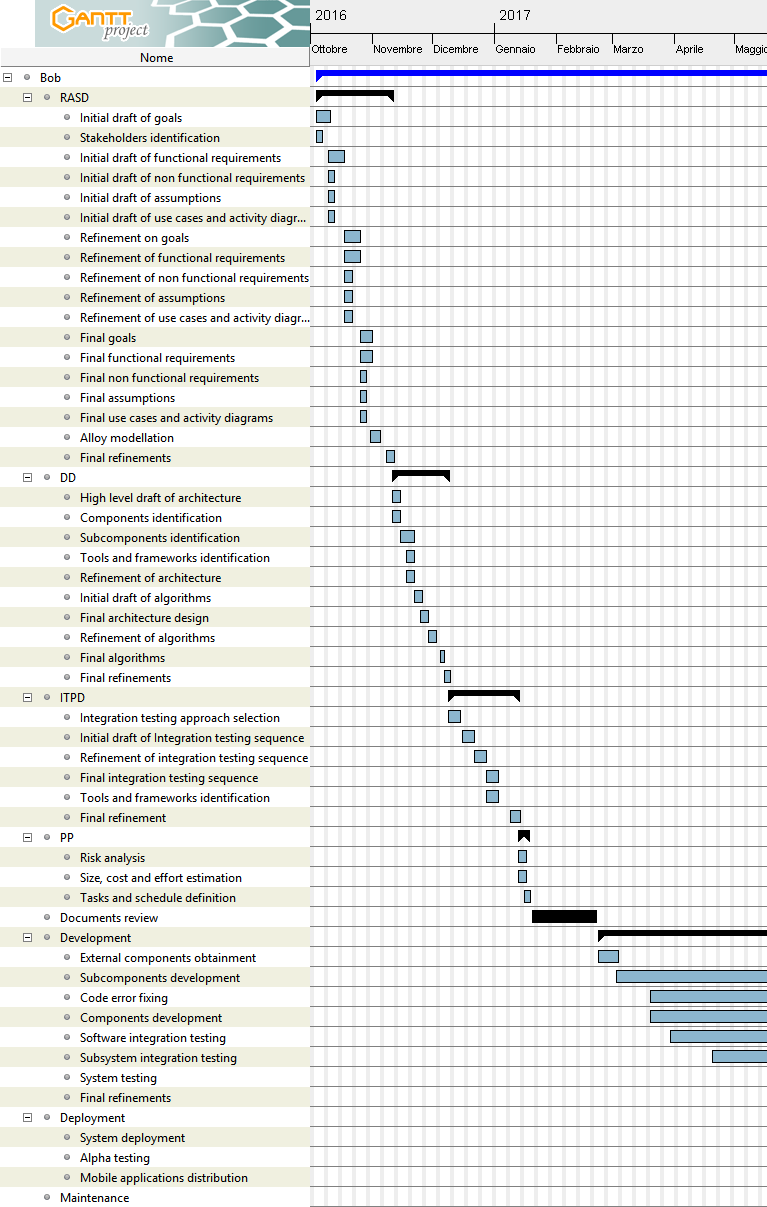
\includegraphics[height=\textheight, keepaspectratio]{resource_allocation/diagrams/ScheduleBob1.png}
\end{figure}

\begin{figure}[H]
	\centering
	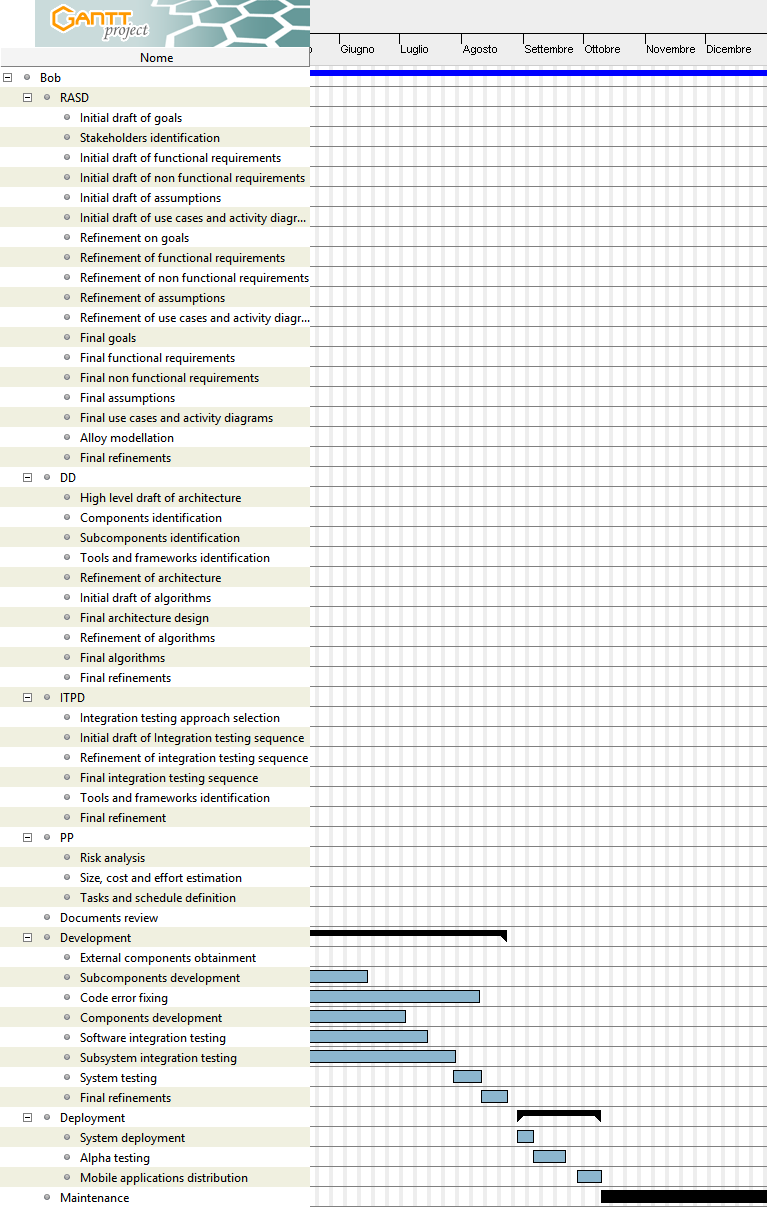
\includegraphics[height=\textheight, keepaspectratio]{resource_allocation/diagrams/ScheduleBob2.png}
\end{figure}

	\section{Risk management}
	
	\section{Appendix}
\subsection{Used tools}
To create the RASD we used the following tools:
\begin{itemize}
	\item \textbf{MikTex} \\ JUnit is a simple framework to write repeatable tests. It is an instance of the xUnit architecture for unit testing frameworks.
 \\ \url{http://junit.org/junit4/} 
	\item \textbf{TexStudio}\\ OpenSource cross-platform LaTeX editor we used to write the RASD. \\ \url{http://texstudio.sourceforge.net/} 
	\item \textbf{StarUML}\\ UML modelling tool we used to build the graphs\\ \url{http://staruml.io/} 
	\item \textbf{Balsamiq}\\ The mockup builder we used to design the mockups. \\ \url{https://balsamiq.com/} 
	\item \textbf{Alloy analyzer 4}\\ used to build  strong and substantial models \\ \url{ http://alloy.mit.edu/alloy/}
	\item \textbf{GitHub desktop}\\ Desktop application of the web-based Git repository hosting service. Used to collaborate in the team and to have a track of the changes.  \\ \url{https://desktop.github.com/} 
\end{itemize}


\subsection{Hours of work}
This is the time spent redacting the RASD
\begin{itemize}
	\item {Lorenzo Binosi} - 80 hours
\end{itemize}

\begin{thebibliography}{1}	
	\bibitem{se-project-rules}
	Software Engineering 2 Project, AA 2016/2017 - \emph{Project goal, schedule and rules}
	
	\bibitem{se-assignment}
	Software Engineering 2 Project, AA 2016/2017 - \emph{Assignments 1}
	
	\bibitem{ieee-830-1198}
	IEEE Standard 830-1998: \emph{IEEE Recommended Practice for Software Requirements Specifications}
	
	\bibitem{w3c-html5}
	W3C, \emph{HTML5 - W3C Recommendation 28 October 2014}, \url{http://www.w3.org/TR/html5/}.
	
	\bibitem{w3c-css}
	W3C, \emph{Cascading Style Sheets Level 2 Revision 1 (CSS 2.1) Specification}, \url{http://www.w3.org/TR/CSS21/}
	
	\bibitem{apple-ios-hig}
	Apple, \emph{iOS Human Interface Guidelines}, \url{https://developer.apple.com/library/ios/documentation/UserExperience/Conceptual/MobileHIG/}
	
	\bibitem{google-android-hig}
	Google, \emph{Android Developers - Design}, \url{https://developer.android.com/design/index.html}
\end{thebibliography}
	
\end{document}